\documentclass{article}

% Compile a preprint version (shows author names). Use [final] for camera-ready.
\usepackage[preprint]{neurips_2024}

\usepackage[utf8]{inputenc} % allow utf-8 input
\usepackage[T1]{fontenc}    % use 8-bit T1 fonts
\usepackage{hyperref}       % hyperlinks
\usepackage{url}            % simple URL typesetting
\usepackage{booktabs}       % professional-quality tables
\usepackage{amsfonts}       % blackboard math symbols
\usepackage{amsmath}
\usepackage{nicefrac}       % compact symbols for 1/2, etc.
\usepackage{microtype}      % microtypography
\usepackage{xcolor}         % colors
\usepackage{graphicx}
\usepackage{fancyhdr}

% Replace the default "Preprint. Under review." first-page notice.
\makeatletter
\renewcommand{\@noticestring}{COMP 514 Final Project Report, Rice University, Fall 2025.}
\makeatother

% Optional first-page footer with author contributions.
% Enable with \thispagestyle{firstpage} right after \maketitle.
\fancypagestyle{firstpage}{%
  \fancyhf{}%
  \renewcommand{\headrulewidth}{0pt}
  \renewcommand{\footrulewidth}{0pt}
  \fancyfoot[C]{%
    \footnotesize
    \textbf{Author contributions:}~
    Ryan Li, Serena You, and Yuanyuan Zhu carried out the project's design,
    implementation, experiments, and presentation preparation.
    Diwesh Chaurasia's involvement was minimal; he did not contribute to the
    codebase or experimental workflow and was unable to attend most meetings
    on time. His only contribution was a short report section drafted with
    GenAI tools, which we have placed in the Appendix for transparency.
  }%
}

\title{Chasing the ``Aha Moment'': A Review and\\
Implementation of Reinforcement Learning\\
in the Post-Training of LLMs}

% NOTE: one author is in the Department of Bioengineering (superscript 2).
% Assign the superscripts to the correct names before submission.
\author{%
  Ryan Li \quad Serena You \quad Yuanyuan Zhu \quad Diwesh Chaurasia \\[4pt]
  Department of Computer Science and Department of Bioengineering\\
  Rice University\\
  \texttt{\{rl182, xy68, yz281, dc162\}@rice.edu}
}

\begin{document}

\maketitle
% \thispagestyle{firstpage}

\begin{abstract}
Reinforcement learning (RL) has become a central ingredient in the post-training of large language models (LLMs). RL-trained models such as DeepSeek-R1 achieve strong reasoning performance, and the DeepSeek-R1 report describes an ``Aha Moment'' in which the model learns to allocate more thinking time by revisiting and revising its initial reasoning. This phenomenon has drawn wide attention in the research community.
In this project, we review RL-based post-training methods for LLMs and implement Group Relative Policy Optimization (GRPO) on Llama~3.1--8B~Instruct under a single-GPU budget. We further design handcrafted reward functions, including a length-based term that rewards longer reasoning when an answer is wrong, to test whether such shaping can elicit behavior similar to the reported Aha Moment.
Our experiments show that the GRPO-trained model performs well on GSM8K but fails on AIME. This contrast suggests that, at the 8B scale, RL does not fundamentally expand a model's underlying capability; it mainly encourages more structured and consistent reasoning. We discuss these findings and outline future work on scaling model size and refining reward design.
\end{abstract}

\section{Introduction}

Large language models (LLMs) have advanced rapidly in recent years and now play a central role in natural language processing, reasoning, and decision-making tasks. Scaling laws show that model capability improves predictably with data and compute \cite{kaplan2020scaling, hoffmann2022chinchilla}, yet post-training has become increasingly important for improving reasoning quality beyond what pretraining and supervised learning alone provide. Among post-training techniques, reinforcement learning (RL) has become a major direction for alignment, instruction following, and step-by-step reasoning \cite{ouyang2022rlhf, ziegler2019fine}.

Recent RL-trained models such as DeepSeek-R1 \cite{deepseekr1} achieve strong results on difficult reasoning benchmarks. A notable observation from that work is the so-called ``Aha Moment'' (Figure~\ref{fig:aha}), in which the model learns, without explicit supervision, to spend more time thinking by revisiting and correcting its initial reasoning. This observation has attracted significant attention because it suggests that RL can shape the reasoning \emph{process} rather than only the final answer.

\begin{figure}[t]
    \centering
    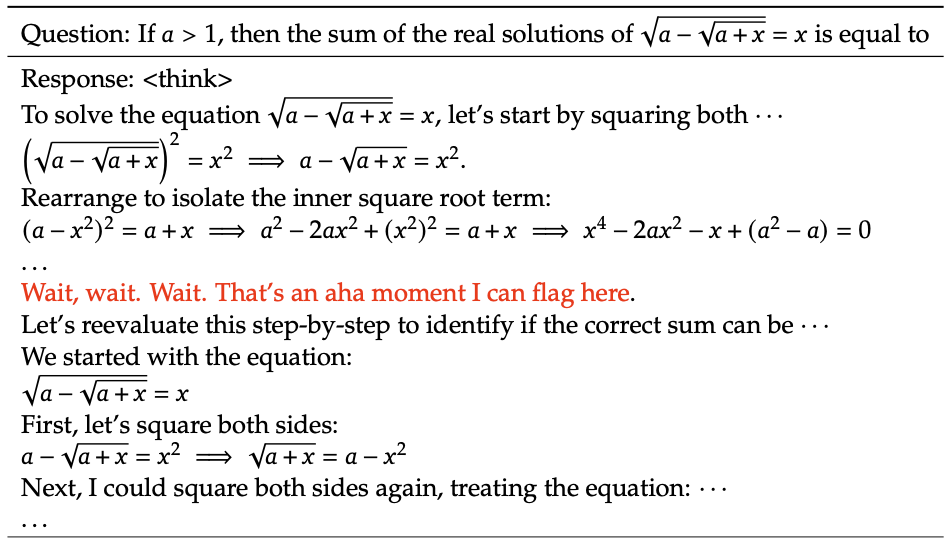
\includegraphics[width=0.95\linewidth]{img/aha_moment_DeepSeek-R1.png}
    \caption{The ``Aha Moment'' reported for DeepSeek-R1-Zero: during RL training, an intermediate checkpoint pauses, re-evaluates its approach, and revises its reasoning. Figure reproduced from the DeepSeek-R1 technical report \cite{deepseekr1}.}
    \label{fig:aha}
\end{figure}

However, the mechanism by which RL improves reasoning remains unclear. Several studies argue that RL-based methods, including RLHF, RLAIF, DPO, and GRPO, do not fundamentally expand a model's representational capacity. Instead, they encourage stability, coherence, and more deliberate reasoning patterns that are already latent in the pretrained model \cite{deepseekr1, r1zero2025, yang2025aha}. Understanding these dynamics matters for designing reward functions that genuinely improve reasoning rather than overfit to shallow heuristics.

In this project, we investigate the role of RL in post-training LLM reasoning. Our contributions are threefold:
\begin{itemize}
    \item We review and summarize existing post-training techniques for LLMs, including supervised fine-tuning (SFT), RLHF, GRPO, and related preference-based and process-based methods.
    \item We implement GRPO on Llama~3.1--8B~Instruct using 4-bit quantization and LoRA on a single NVIDIA T4 GPU, and we design handcrafted reward functions intended to encourage deeper reflection and potentially trigger Aha-Moment-like behavior.
    \item We evaluate the trained model on GSM8K and AIME. RL improves GSM8K accuracy by about 2.4 percentage points (82.6\% to 85.0\%) but does not transfer to AIME, supporting the hypothesis that RL encourages longer and more consistent chains of thought without increasing the inherent reasoning ability of the model.
\end{itemize}

These findings motivate our future work. We plan to scale up the base model and to explore whether more structured reward functions can meaningfully improve high-level mathematical reasoning, which may shed light on the limits of RL-based post-training and its interaction with model capacity.

Our code, training notebooks, and this report are available at \url{https://github.com/Ryanrc03/Chasing-the-Aha-Moment}.

\section{Related Work}

\subsection{Supervised Fine-Tuning}

Supervised fine-tuning (SFT) is the foundational post-training step used to align pretrained language models with human-preferred behavior. Popularized by InstructGPT \cite{ouyang2022rlhf}, SFT trains on curated prompt--response pairs with a next-token prediction objective, so the model learns to imitate high-quality demonstrations in both content and structure. Instruction-tuned systems such as Llama~3~Instruct \cite{llama3} show that SFT reliably turns a pretrained LLM, whose outputs often resemble uncontrolled text continuation, into a capable instruction follower with improved coherence, formatting, and task adherence. Because SFT requires neither a reward model nor preference comparisons, it remains the most stable and widely used first stage in modern LLM pipelines.

\paragraph{Stabilizing the model before RL.}
A key role of SFT in the DeepSeek-R1 pipeline is to stabilize the model before reinforcement learning. The authors report that DeepSeek-R1-Zero, trained purely with RL from the base model, frequently produced unreadable chains of thought, fragmented or looping sentences, and mixed English--Chinese token streams \cite{deepseekr1}. These issues indicate that RL applied directly to a pretrained model can amplify noise and stylistic inconsistencies rather than produce meaningful improvement. A small amount of ``cold-start'' SFT lets DeepSeek-R1 avoid such degenerate behavior: the model learns clean formatting, coherent multi-sentence reasoning, and a consistent separation between the reasoning process and the final summary, giving RL a well-structured linguistic foundation.

\paragraph{Providing a reasoning scaffold.}
Although SFT does not itself induce the Aha Moment, it establishes the structural scaffold on which such behavior can emerge. Through demonstrations of step-by-step explanations and final summaries, SFT teaches the model the \emph{format} of a reasoning process, even if the model does not yet refine or critique its own steps. DeepSeek-R1 formalizes this scaffold with a template that has explicit reasoning and summary regions. RL then uses the scaffold to encourage self-correction, re-evaluation, and adaptive thinking depth. In this sense, SFT provides the grammatical and organizational framework within which RL can later induce reflective reasoning.

\paragraph{Limitations.}
SFT is fundamentally imitation-based and therefore has intrinsic limits. Because it optimizes only the likelihood of demonstrated outputs, it does not reward deeper reasoning, exploration, or alternative solution strategies. It cannot teach a model to reflect on or correct its own mistakes, nor to modulate thinking time according to task difficulty. SFT-trained models also tend to overfit the stylistic patterns of the demonstration data, which limits their ability to discover new reasoning approaches. For these reasons, SFT alone is insufficient for producing emergent behaviors such as the Aha Moment, motivating preference-based and reinforcement-based methods that optimize reasoning quality rather than pure imitation.

\subsection{Reinforcement Fine-Tuning}

The 2017 work of Christiano et al.\ \cite{christiano2017deep}, which first used human preference signals to train a reward model that then guides policy optimization, is widely regarded as the conceptual origin of reinforcement fine-tuning (RFT). Instead of hand-crafted reward signals, it collects pairwise comparisons of short trajectory segments from human evaluators, trains a reward model on these comparisons, and uses that model to guide an RL agent. Building on this framework, Ziegler et al.\ \cite{ziegler2019fine} showed that the same methodology extends to large language models, giving rise to the RLHF pipeline widely used today: collect human preference data, fit a reward model, and optimize the policy with Proximal Policy Optimization (PPO) under a KL penalty that keeps updates stable. This work established RLHF as a practical and effective method for aligning language models with human expectations \cite{ouyang2022rlhf, bai2022training}.

Modern RFT methods extend RLHF with more stable, reward-model-free, and compute-efficient optimization schemes that better support large-scale reasoning. Among them, Group Relative Policy Optimization (GRPO) \cite{shao2024deepseekmath} is a central development. GRPO samples a group of candidate solutions for each problem, scores them with task-specific correctness signals, and uses the group statistics as a baseline, which removes the need for a separate value network and reduces the training instability commonly seen in PPO-style RLHF. In DeepSeekMath and DeepSeek-R1, GRPO is applied as a reinforcement fine-tuning stage after supervised learning to strengthen multi-step mathematical reasoning \cite{shao2024deepseekmath, deepseekr1}. Figure~\ref{fig:rlhf-pipeline} gives an overview of the general RL-for-LLM framework.

More generally, RFT improves a model by training on a reward signal rather than only on labeled data. The model produces multiple candidate responses, which are assessed by human feedback, AI feedback, deterministic correctness checks, or group-wise ranking. These assessments yield scalar or relative rewards that are converted into advantages for policy-gradient updates such as PPO or GRPO. Through repeated updates, the model increases the likelihood of high-quality reasoning trajectories and better-aligned outputs.

\begin{figure}[t]
    \centering
    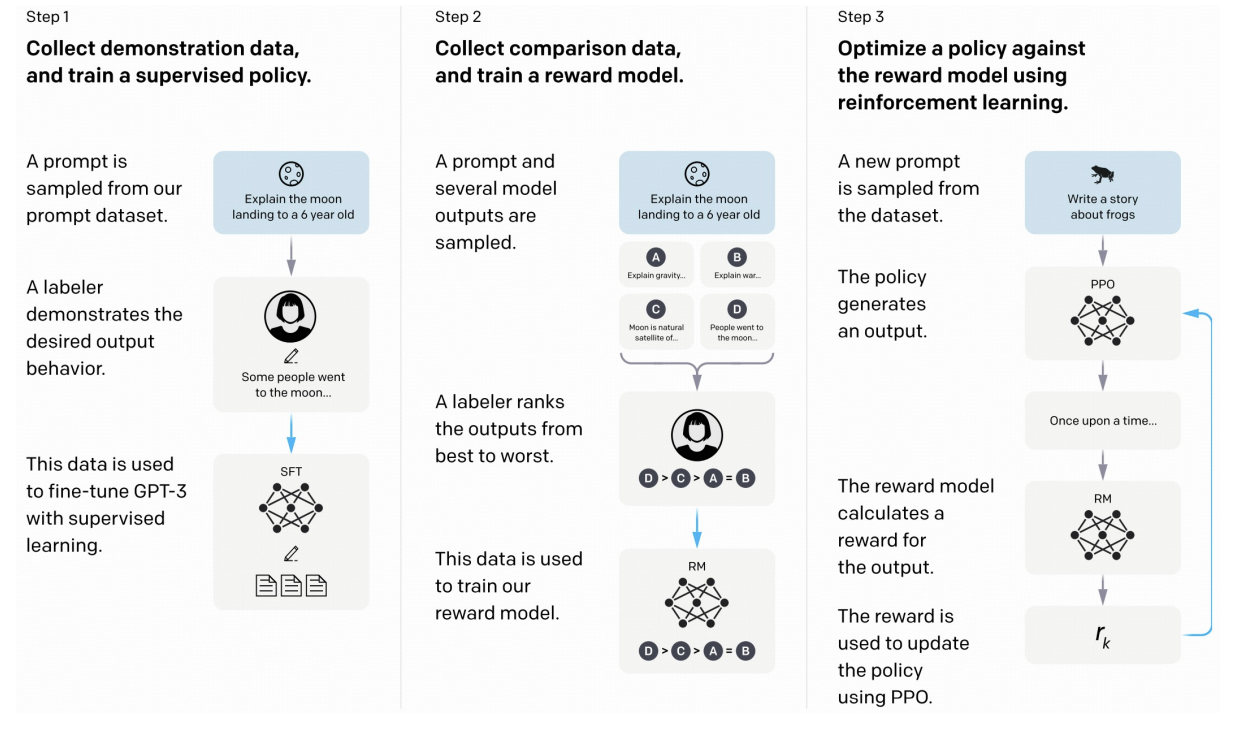
\includegraphics[width=\linewidth]{img/frame_work.png}
    \caption{Overview of the RL-for-LLMs framework. Adapted from \emph{Reinforcement Learning Enhanced LLMs: A Survey} \cite{wang2025rlsurvey}.}
    \label{fig:rlhf-pipeline}
\end{figure}

\paragraph{Advantages and disadvantages.}
RFT can incorporate evaluative feedback, whether from humans, AI feedback models, or deterministic verifiers, into a principled optimization framework. This lets it optimize behaviors that supervised learning cannot easily capture, such as multi-step reasoning, self-correction, tool use, and structured task completion. On the other hand, RLHF-style RFT requires large amounts of human preference data, making it expensive and sensitive to annotation quality \cite{bai2022training}. Learned reward models are prone to over-optimization, where the policy exploits weaknesses of the reward model rather than genuinely improving, leading to instability and reward hacking \cite{rafailov2024scaling}. Even reward-model-free variants incur substantial compute, because they need multiple samples per prompt and additional evaluation overhead. Finally, the policy-gradient nature of RFT brings optimization challenges, including sensitivity to hyperparameters and reduced output diversity when preference shaping becomes too strong \cite{rafailov2024scaling}.

\paragraph{Cost.}
The cost of RFT arises from data collection, sampling, evaluation, and policy optimization. Among SFT, RLHF, and GRPO, RLHF is the most expensive: it relies on large-scale human preference data and a separately trained reward model, and the policy must repeatedly query that reward model during PPO updates, creating a two-model training loop \cite{bai2022training, rafailov2024scaling}. GRPO reduces cost substantially by eliminating the reward model. It replaces a learned reward function with deterministic correctness signals or group-wise rankings over sampled outputs, removing the need for human annotators and reward-model training, which is what makes it feasible on a single consumer-grade GPU as in this project.

\subsection{Reproducing the Aha Moment at Small Scale}

Several recent works ask whether Aha-Moment-like behavior can be reproduced in much smaller models through RL post-training. Zhou et al.\ \cite{r1zero2025} report self-reflective reasoning emerging in a 2B non-SFT multimodal model trained with GRPO. TinyLLaVA-Video-R1 \cite{tinyllava2025} applies RL to a 4B video model and observes reflective reasoning and ``rethinking'' during training. SimpleRL-Zoo \cite{simplerlzoo} studies zero-RL training across ten open base models from 0.5B to 32B parameters and finds that increases in response length and reflective phrases appear in several of them, while also cautioning that such surface signals do not always coincide with accuracy gains. Yang et al.\ \cite{yang2025aha} analyze Aha Moments from the perspective of internal mechanisms and argue that they reflect changes in how the model allocates computation rather than new knowledge. These works motivate our attempt to elicit similar behavior in an 8B model under a tight compute budget.

\section{Methodology}

In this section we describe the output format and the notion of ``reasoning'' used throughout our experiments, the GRPO objective that connects rewards to model updates, and the reward design we use to encourage reflective behavior.

\subsection{Reasoning as Rewarded Trajectories}

Following chain-of-thought (CoT) prompting \cite{wei2022cot, kojima2022zeroshot}, we structure the model's output as an explicit reasoning trace followed by a final answer. For a question $x$ the model generates $y = (z, a)$, where $z$ is the chain-of-thought segment and $a$ is the final answer. In practice we realize this structure with XML-style tags:
\begin{equation}
    y \;=\; \texttt{<reasoning>}\; z \;\texttt{</reasoning><answer>}\; a \;\texttt{</answer>}.
\end{equation}
At evaluation time we parse $a$ from the \texttt{<answer>} tag and compare it with the gold answer, while $z$ is used to analyze reasoning behavior such as the length and stability of the chain of thought.

We treat the language model as a policy $\pi_{\theta}(\cdot \mid x)$ that samples trajectories $\tau = (z, a)$, and we score each trajectory with a scalar reward
\begin{equation}
    R(x,\tau) \;=\; R_{\text{acc}}(x,a) \;+\; R_{\text{format}}(x,\tau) \;+\; R_{\text{len}}(x,z),
    \label{eq:reward}
\end{equation}
where $R_{\text{acc}}$ rewards a correct final answer, $R_{\text{format}}$ rewards well-formed XML structure with a clean separation between reasoning and answer, and $R_{\text{len}}$ is a length-based term, defined in Section~\ref{sec:len}, that encourages longer and more deliberate reasoning when the model would otherwise terminate prematurely or answer incorrectly. ``Reasoning'' is thus operationalized as the set of trajectories that obtain high reward under $R$, rather than as a separate symbolic module.

In our implementation, $R_{\text{acc}}$ gives $2.0$ for an exact match with the gold answer and an additional $0.5$ when the extracted answer is an integer. $R_{\text{format}}$ is the sum of a strict and a soft regular-expression match on the tag structure ($0.5$ each) and a fine-grained tag-count term that awards $0.125$ per correctly placed tag and penalizes trailing text after \texttt{</answer>}.

\subsection{GRPO-Based Fine-Tuning}

To connect the reward to model updates we adopt Group Relative Policy Optimization (GRPO) \cite{shao2024deepseekmath}, a variant of PPO that removes the need for a separate value network. For each question $x$ we sample a group of $K$ candidate trajectories $\{\tau_{k}\}_{k=1}^{K}$ from the old policy $\pi_{\theta_{\text{old}}}(\cdot \mid x)$ and compute their rewards $r_{k} = R(x, \tau_{k})$. GRPO uses the group mean as a baseline,
\begin{equation}
    \bar{r} \;=\; \frac{1}{K} \sum_{k=1}^{K} r_{k},
    \qquad
    A_{k} \;=\; r_{k} - \bar{r},
\end{equation}
and optimizes a clipped sequence-level objective
\begin{equation}
    J_{\text{GRPO}}(\theta)
    \;=\;
    \mathbb{E}_{x}
    \biggl[
        \frac{1}{K} \sum_{k=1}^{K}
        \min \Bigl(
            \rho_{k}(\theta) A_{k},
            \operatorname{clip}\bigl(\rho_{k}(\theta), 1 - \varepsilon, 1 + \varepsilon\bigr) A_{k}
        \Bigr)
    \biggr],
\end{equation}
where
\begin{equation}
    \rho_{k}(\theta)
    \;=\;
    \frac{\pi_{\theta}(\tau_{k} \mid x)}{\pi_{\theta_{\text{old}}}(\tau_{k} \mid x)}
\end{equation}
is the importance ratio between the current and old policies and $\varepsilon$ is the clipping hyperparameter. Intuitively, GRPO raises the probability of trajectories whose reward exceeds the group average and lowers that of trajectories below it, while clipping stabilizes the update. The original formulation also normalizes $A_k$ by the group standard deviation and adds a KL penalty toward a reference policy; we follow the TRL implementation, which includes both.

\subsection{Length-Based Reward Shaping}
\label{sec:len}

One of the most salient empirical signatures of the Aha Moment is the emergence of longer and more deliberate chains of thought, especially when the model's initial attempt is incorrect. To encourage such reflective behavior explicitly, we augment the reward with a length-based component that depends on the chain-of-thought segment $z$.

Let $\ell(z)$ be the length of $z$ in tokens and $L_{\max}$ a fixed truncation threshold. We define the normalized length
\begin{equation}
    \tilde{\ell}(z) \;=\; \min\!\Bigl(\frac{\ell(z)}{L_{\max}},\, 1\Bigr) \in [0,1],
\end{equation}
which measures how close the reasoning trace is to the target length scale. Writing $\mathbb{I}(\cdot)$ for the indicator function and treating $R_{\text{acc}}$ as a binary correctness signal, the length-based term is
\begin{equation}
    R_{\text{len}}(x, z)
    \;=\;
    \alpha \, \mathbb{I}\!\bigl(R_{\text{acc}}(x,a) = 0\bigr)\, \tilde{\ell}(z)
    \;-\;
    \beta \, \mathbb{I}\!\bigl(R_{\text{acc}}(x,a) = 1\bigr)\, \tilde{\ell}(z),
\end{equation}
with hyperparameters $\alpha > 0$ and $\beta \ge 0$.

When the final answer is wrong, the model receives a bonus proportional to the normalized CoT length, which encourages it to allocate more ``thinking time'' by extending its reasoning. When the answer is already correct, overly long chains of thought are mildly penalized, which discourages unbounded verbosity. The overall reward in Equation~\ref{eq:reward} therefore encodes a preference for reflective behavior: in failure states the model is pushed toward deeper reasoning, and in success states it is nudged toward concise but well-structured solutions. In practice we choose modest values of $\alpha$ and $\beta$ so that $R_{\text{len}}$ shapes the trajectory without overwhelming the accuracy signal.

\section{Experiments}

\subsection{Experimental Setup}

All experiments run in Google Colab on a single NVIDIA T4 GPU with 15\,GB of memory. Our policy is Llama~3.1--8B~Instruct \cite{llama3} loaded through Unsloth \cite{unsloth} in 4-bit quantization \cite{dettmers2023qlora}, with a rank-32 LoRA adapter \cite{hu2022lora} on all attention and feed-forward projections (about 84M trainable parameters, or 1\% of the model). Generation during training uses vLLM~0.9.2 co-located with the trainer, and policy updates use the GRPO implementation in TRL~0.22.2 \cite{trl} with PyTorch~2.7 and CUDA~12.6.

Table~\ref{tab:hparams} lists the main hyperparameters. We sample six completions per prompt, cap prompts at 256 tokens and completions at 768 tokens, and train for 250 steps with 8-bit paged AdamW, a learning rate of $5\times10^{-6}$ with cosine decay and 10\% warm-up, and gradient clipping at 0.1. Random seeds are fixed. Despite the limited hardware, this configuration reliably supports controlled studies of GRPO and reward shaping.

\begin{table}[t]
\centering
\begin{tabular}{ll}
\toprule
\textbf{Setting} & \textbf{Value} \\
\midrule
Base model & Llama~3.1--8B~Instruct, 4-bit \\
LoRA rank / $\alpha$ & 32 / 32 \\
LoRA targets & q, k, v, o, gate, up, down projections \\
Generations per prompt ($K$) & 6 \\
Max prompt / completion length & 256 / 768 tokens \\
Optimizer & paged AdamW (8-bit), $\beta_1{=}0.9$, $\beta_2{=}0.99$, wd 0.1 \\
Learning rate & $5\times10^{-6}$, cosine, 10\% warm-up \\
Gradient clipping & 0.1 \\
Training steps & 250 \\
\bottomrule
\end{tabular}
\medskip
\caption{GRPO training configuration used in all experiments.}
\label{tab:hparams}
\end{table}

\subsection{Datasets}

All experiments use public mathematical reasoning datasets. For RL training we use the \texttt{openai/gsm8k} training split \cite{cobbe2021gsm8k}, converting each example into a chat-style prompt with the system instruction that specifies the XML output format, and extracting the gold answer after the \texttt{\#\#\#\#} marker. GSM8K's concise, well-structured grade-school word problems make it an effective setting for studying small-model RL.

For evaluation we use two benchmarks: (1) the full GSM8K test split (1{,}319 problems) to measure in-distribution performance, and (2) a combined AIME set of 60 problems, consisting of AIME~2024 and AIME~2025 (parts I and II), to assess out-of-distribution generalization.\footnote{\texttt{HuggingFaceH4/aime\_2024} and \texttt{opencompass/AIME2025} on the Hugging Face Hub.} AIME problems are substantially harder and require longer and more precise reasoning chains. Evaluation uses greedy-leaning sampling (temperature 0.2, top-$p$ 0.95) with up to 512 generated tokens, and we report accuracy after numeric normalization of the extracted answer, the rate at which an \texttt{<answer>} tag could be parsed, and the rate at which the full \texttt{<reasoning>}/\texttt{<answer>} structure was matched.

\subsection{Instruct Baseline vs.\ GRPO}

The instruction-tuned starting point already provides a useful initialization for mathematical reasoning, but its behavior is limited by exposure bias and the absence of explicit reasoning supervision. In our experiments the baseline model often produces verbose or meandering explanations, switches solution strategies within a single response, or introduces unnecessary computational methods. Although it generates mathematically relevant text, it frequently fails to deliver a stable, well-formed final answer in the required \texttt{<answer>} format, treating the task as open-ended text generation rather than goal-directed problem solving.

GRPO changes this behavior substantially. Unlike SFT, which optimizes next-token prediction, GRPO directly reinforces correct final answers and a structured output format and penalizes inconsistent intermediate reasoning. Even a small amount of GRPO training yields noticeable improvements: the model becomes more concise, takes fewer detours in its reasoning, and reliably terminates with a correctly formatted answer. GRPO also reduces generation variability, making the model less prone to contradictory steps or mid-solution strategy changes. These gains appear despite the strict memory constraints of a single T4 GPU, which shows that reward-driven alignment can be effective at small scale.

Qualitatively, GRPO produces behavior reminiscent of the ``micro-aha'' phenomenon discussed in recent work on RL-enhanced LLMs. Whereas the baseline occasionally attempts several reasoning paths within one response, the GRPO-trained model follows a more deliberate pattern: it selects a single method, applies it consistently, and stays aligned with the task objective. This contrast is especially clear in our pi-calculation case study (Table~\ref{tab:pi}), where the baseline gives long pedagogical explanations or switches algorithms mid-solution, while the GRPO-trained model follows one coherent line of reasoning and outputs a precise, well-structured final answer. Together, these observations highlight the role of reinforcement feedback in stabilizing reasoning behavior and improving task adherence beyond what SFT alone provides.

\begin{table}[t]
\centering
\begin{tabular}{p{0.95\linewidth}}
\toprule
\textbf{Instruct baseline (no GRPO)} \\
\midrule
\texttt{``Calculating pi is a classic mathematical challenge. There are various methods to calculate pi, but I'll use the most common and simple one, the Leibniz formula...''} \\
The model outputs two different Python implementations (Leibniz series and Gauss--Legendre), discusses convergence, and adds extended mathematical commentary. No final numerical answer is given in the required \texttt{<answer>} format. \\
\midrule
\textbf{GRPO-trained model} \\
\midrule
\texttt{``Unfortunately, calculating the exact value of pi is a complex task... However, we can approximate it using the Leibniz series...''} \\
The model gives a concise explanation, a single coherent Python snippet, and a final answer in the required structured format: \\
\quad\texttt{<answer>3.141592653589793</answer>} \\
\bottomrule
\end{tabular}
\medskip
\caption{Qualitative comparison before and after GRPO training on the prompt ``Calculate pi.'' Without GRPO the model rambles, switches methods mid-solution, and fails to produce a structured answer. After GRPO it selects one method, follows a stable reasoning pattern, and reliably closes with a clean \texttt{<answer>} tag.}
\label{tab:pi}
\end{table}

\subsection{Rewarding Reflective CoT Expansion}

Prior studies of the Aha Moment observe that models shift into longer and more deliberate chains of thought when their initial reasoning appears incorrect, a behavior interpreted as a self-reflective adjustment that allocates extra thinking time. Motivated by this, we test whether the length-based reward of Section~\ref{sec:len} can encourage a similar reflective response in an 8B model.

Tables~\ref{tab:gsm8k} and \ref{tab:aime} compare GRPO with the base reward ($R_{\text{acc}} + R_{\text{format}}$) against GRPO with the full shaped reward of Equation~\ref{eq:reward}. On GSM8K, reward shaping raises accuracy from 82.6\% to 85.0\% and increases the fraction of outputs matching the complete \texttt{<reasoning>}/\texttt{<answer>} structure from 0\% to 23\%, at the cost of a small increase in generation latency, consistent with longer reasoning traces. The near-perfect XML parse rate in both settings shows that the baseline reward already teaches the model to emit an \texttt{<answer>} tag; the shaped reward is what makes the surrounding reasoning structure consistent.

\begin{table}[t]
\centering
\begin{tabular}{lcc}
\toprule
\textbf{Metric} & \textbf{GRPO (base reward)} & \textbf{GRPO + reward shaping} \\
\midrule
GSM8K test samples         & 1{,}319 & 1{,}319 \\
Accuracy                   & 0.8256 & \textbf{0.8500} \\
XML parse rate             & 1.0000 & 0.9980 \\
Format (soft)              & 0.0000 & \textbf{0.2300} \\
Avg.\ latency (s / sample) & 5.56   & 5.84   \\
Wall-clock time (s)        & 7{,}329 & 7{,}700 \\
\bottomrule
\end{tabular}
\medskip
\caption{Effect of reward shaping on the GSM8K test set. The shaped reward yields a modest but consistent accuracy gain and a large gain in format compliance, with slightly higher generation latency.}
\label{tab:gsm8k}
\end{table}

\begin{table}[t]
\centering
\begin{tabular}{lcc}
\toprule
\textbf{Metric} & \textbf{GRPO (base reward)} & \textbf{GRPO + reward shaping} \\
\midrule
AIME samples                & 60      & 60      \\
Accuracy                    & 0.0000  & 0.0000  \\
XML parse rate              & 1.0000  & 0.9833  \\
Format (soft)               & 0.0333  & \textbf{0.1167} \\
Avg.\ latency (s / sample)  & 14.26   & 15.48   \\
Wall-clock time (s)         & 422.3   & 456.0   \\
\bottomrule
\end{tabular}
\medskip
\caption{GRPO with and without reward shaping on the combined AIME 2024 and 2025 set. Neither model solves any problem, reflecting the extreme difficulty and out-of-distribution nature of olympiad problems for an 8B model. Reward shaping nevertheless increases format consistency and generation time, indicating more structured and deliberate chains of thought even when the problems are not solved.}
\label{tab:aime}
\end{table}

\subsection{Why GRPO Does Not Transfer to AIME}

Despite clear improvements on GSM8K, our GRPO-trained 8B model does not generalize to AIME 2024/2025, where accuracy stays at zero. Although both benchmarks involve mathematical reasoning, AIME problems require multi-step symbolic manipulation, non-linear algebra, and olympiad-level abstraction far outside the GSM8K distribution. The absence of correct answers does not mean the model has not changed: we observe more deliberate chains of thought and consistently well-formed XML output. The model attempts deeper reasoning but lacks the capacity to complete these problems.

This matches common critiques of GRPO and related RL approaches: they refine and stabilize the model's existing reasoning behavior but do not expand its underlying algorithmic or representational ability. In effect, GRPO enforces more consistent reasoning trajectories without creating new mathematical competence, an inherent limitation at the 8B scale. The poor AIME performance therefore reflects the constraints of model scale and training budget rather than a flaw in the reward design. Larger models trained with GRPO or R1-style methods show more transferable reasoning, likely because of richer inductive biases and stronger latent mathematical priors. Within the small-model regime, our results mark a realistic boundary: GRPO can encourage more thoughtful reasoning, but it cannot compensate for insufficient capacity on high-difficulty tasks.

\subsection{Discussion and Future Work}

The sharp contrast between gains on GSM8K and zero accuracy on AIME highlights a core limitation of small LLMs trained with RL: RL improves consistency but does not expand the model's underlying reasoning capacity. GSM8K lies close to the pretraining distribution, whereas AIME demands multi-step symbolic manipulation and olympiad-level abstraction. Prior work \cite{r1zero2025, deepseekr1, simplerlzoo} similarly finds that GRPO-like methods stabilize existing reasoning patterns without enabling fundamentally new capabilities.

This gap indicates that reward shaping alone cannot bridge the distributional jump from grade-school to olympiad mathematics. Model scale and pretraining depth appear decisive, as larger R1-style or process-supervised models \cite{deepseekr1, wang2025rlsurvey} exhibit more transferable reasoning. Scaling our experiments to 13B--70B checkpoints would clarify whether the benefits we observe persist beyond GSM8K.

A complementary direction is \emph{process-level reward} \cite{lightman2023verify}, which offers denser supervision and may help smaller models build more verifiable reasoning chains. Synthetic data, self-play, and bootstrapping \cite{deepseekr1, r1zero2025, kojima2022zeroshot} could further enrich the training distribution and narrow the gap. Our own training budget (250 GRPO steps, roughly one GPU-hour) is also small; longer runs with more generations per prompt and longer completion limits are a natural next step, and we are preparing a follow-up run that compares a 3B base model trained for longer against the present 8B setting.

In summary, while GRPO improves structure and stability, our results reinforce that scale remains the dominant driver of out-of-distribution mathematical reasoning. Combining larger models, process-based rewards, and richer reasoning curricula may yield more generalizable improvements.

\bibliographystyle{unsrt}
\bibliography{references}

\appendix
\section{Unused Related Work Draft (Contributed by Diwesh Chaurasia)}

\emph{The following section was drafted for an earlier version of the project plan that included SFT and DPO stages. Those stages were not run in the final experiments; the text is included unchanged for transparency.}

\subsection{Supervised Fine-Tuning (SFT)}

Supervised Fine-Tuning (SFT) serves as the initial stage of our post-training pipeline and provides the baseline behavior from which later reinforcement-based methods build. Before applying DPO or RFT, we fine-tune the base Llama~3.1--8B model on high-quality reasoning demonstrations to establish stable output formatting, mathematical coherence, and initial chain-of-thought capabilities.

\subsubsection*{Training Setup}

For SFT, we fine-tuned the model using GSM8K-style reasoning samples formatted in our XML chain-of-thought structure:
\begin{quote}
\texttt{<reasoning> ... </reasoning>} \\
\texttt{<answer> ... </answer>}
\end{quote}

This formatting is essential because later reinforcement learning stages rely on clean extraction of the reasoning and answer segments when computing rewards such as accuracy, formatting compliance, and chain-of-thought length. The model is fine-tuned using LoRA adapters (rank 64) applied to the quantized Llama~3.1--8B backbone, enabling training within the memory constraints of a single NVIDIA T4 GPU.

\subsubsection*{Training Objective}

The SFT objective follows standard next-token prediction:
\[
L_{\text{SFT}}(\theta) =
-\mathbb{E}_{(x,y) \sim D_{\mathrm{SFT}}}
\sum_{t=1}^{T} \log p_\theta(y_t \mid x, y_{<t}).
\]

This stage teaches the model to reproduce multi-step reasoning sequences, adhere to structured tagging conventions, and generate mathematically coherent solution steps. Importantly, SFT helps the model internalize the general style of chain-of-thought reasoning that later RL-based methods reinforce more explicitly.

\subsubsection*{Behavior After SFT}

While SFT improves intermediate reasoning quality, we observe several limitations:
\begin{itemize}
    \item The model often produces verbose or drifting reasoning traces.
    \item It treats the answer as open-ended text and may fail to terminate cleanly with the required \texttt{<answer>} tag.
    \item Final answers may still be missing or incorrect despite coherent reasoning steps.
\end{itemize}

These observations reflect known issues in SFT-only training, where imitation provides structure but cannot enforce correctness or stability.

\subsubsection*{Role of SFT in the Post-Training Pipeline}

Although SFT does not induce ``Aha Moment'' reasoning, it plays a critical foundational role:

\begin{enumerate}
    \item \textbf{Stable Initialization:} Reinforcement-based optimization such as GRPO is sensitive to initialization; SFT ensures the model already understands structured reasoning.
    \item \textbf{Format Conditioning:} Reward functions rely on clean extraction of reasoning and answer segments; SFT teaches the XML structure used later by RFT.
    \item \textbf{Preliminary Reasoning Ability:} SFT provides basic multi-step reasoning patterns that RL-based methods refine into more stable and concise forms.
\end{enumerate}

Thus, SFT establishes the groundwork necessary for effective alignment and consistency in later stages such as DPO and RFT.

\subsection{Direct Preference Optimization (DPO)}

In this section, we describe how we applied \textbf{Direct Preference Optimization (DPO)}~\cite{rafailov2023dpo} as a post-training method for our small-scale language model (quantized Llama~3.1--8B with LoRA adapters), and our rationale for using it in the context of enhancing reasoning stability.

\subsubsection*{Motivation for DPO}

Traditional RLHF pipelines require training a separate reward model and running reinforcement learning. DPO provides a simpler, more efficient approach by directly optimizing the model to prefer human-preferred outputs over less desirable ones using a pairwise preference loss. Given our compute limits (single T4 GPU, 4-bit quantization, LoRA rank 64), DPO is an appealing choice for improving reasoning behavior.

\subsubsection*{Implementation}

We constructed a preference dataset consisting of GSM8K prompts paired with multiple candidate completions. These completions were ranked based on:
\begin{itemize}
    \item correctness of the final answer,
    \item clarity and structure of the reasoning chain,
    \item compliance with the XML-style formatting.
\end{itemize}

Training used the standard DPO loss. For each prompt $x$, preferred output $y_w$, and non-preferred output $y_l$, we optimize:
\[
\log \sigma\Bigl(
\beta \log \frac{\pi_\theta(y_w \mid x)}{\pi_{\text{ref}}(y_w \mid x)}
-
\beta \log \frac{\pi_\theta(y_l \mid x)}{\pi_{\text{ref}}(y_l \mid x)}
\Bigr),
\]
where $\pi_{\text{ref}}$ is a frozen reference model.

We reused LoRA rank 64 applied to attention and feedforward layers to stay within memory constraints.

\subsubsection*{Observations and Role in ``Aha Moment'' Investigation}

After DPO fine-tuning, we observed:
\begin{itemize}
    \item clearer structure in chain-of-thought traces,
    \item more stable and consistent reasoning patterns,
    \item improved formatting adherence,
    \item better---but still limited---final-answer accuracy.
\end{itemize}

DPO encourages preferred reasoning styles but does not fundamentally expand reasoning capabilities. It improves discipline and stability, serving as a complementary step before reinforcement-based optimization such as RFT or GRPO.

\subsubsection*{Conclusion}

DPO offered a lightweight, resource-efficient alignment method that strengthened clarity, structure, and consistency in outputs. While it does not directly induce ``Aha Moment'' reasoning or enable out-of-distribution generalization, it meaningfully stabilizes reasoning patterns in preparation for more advanced post-training stages.

\end{document}
